\section{State of the art}

Robots that interact with humans have been developped since the mid-twentieth century. Here is a list of some of the most relevant robots to the field of application of the PD-SD built to date. 


\subsection{SAM/Robonaut}
Built in 1969, the Self-propelled Anthropomorphic Manipulator (SAM), seen in Figure \ref{sam}, was NASA's first radio teleoperated robot. It was composed of two distinct parts: the manipulator and the control center.\\

The manipulator consisted of a torso with two arms and a camera attached to a four wheeled base. The robot sent video feed from the camera over a radio to the operator which would receive the video on a television set.\\

	\begin{figure}[H]
			\centering
			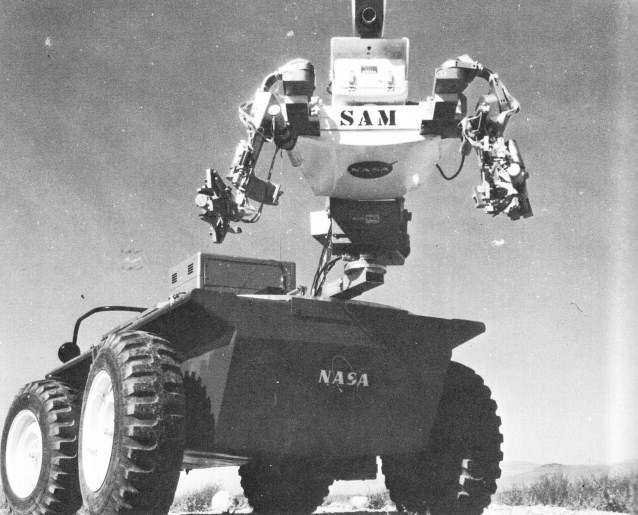
\includegraphics[scale=0.5]{images/StateOfArt/SAM.jpg}
			\caption{NASA's Self-propelled Anthropomorphic Manipulator }
			\label{sam}
	\end{figure}
	\bigskip

The control station, as seen in Figure \ref{sam2}, included an upper-body exoskeleton through which the operator could move their arms and have the robot replicate the movements and the screen through which the robot displayed the video stream.\\

	\begin{figure}[H]
			\centering
			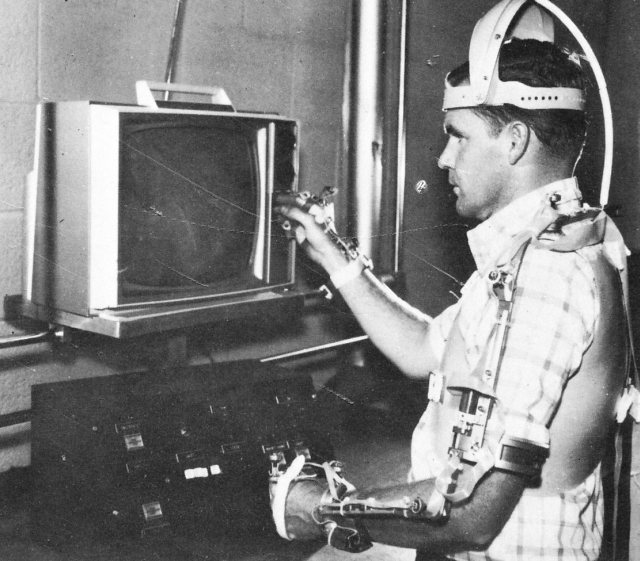
\includegraphics[scale=2]{images/StateOfArt/SAM2.jpg}
			\caption{SAM's control station }
			\label{sam2}
	\end{figure}
	
In the year 1997 NASA started developping Robonaut, a teleopresence robot that would assist astronauts in tasks too dangerous or mundane for them to work on. The combination of the four wheeled base Centaur with Robonaut creates a powerful, efficient, fast successor of the original SAM, while providing a much smaller, portable control station (Figure \ref{robonaut}).

	\begin{figure}[H]
			\centering
			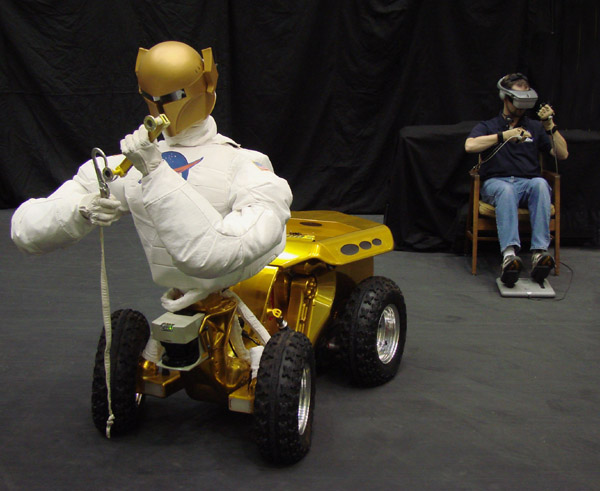
\includegraphics[scale=0.55]{images/StateOfArt/robonaut.jpg}
			\caption{Operator controlling the Robonaut coupled to the Centaur}
			\label{robonaut}
	\end{figure}
	\bigskip 

%\subsection{Asibot}

\subsection{Asimo}

Introduced in the year 2000, Honda's Advanced Step in Innovative MObility (ASIMO) is a humanoid robot designed to assist humans in daily tasks. Its height of 130cm ensures it is able to operate door handles and light switches. Capable of recognizing voice commands and common gestures such as pointing or waving as well as different human faces, the robot is capable of facing and interacting with whoever is speaking. \\


	\begin{figure}[H]
			\centering
			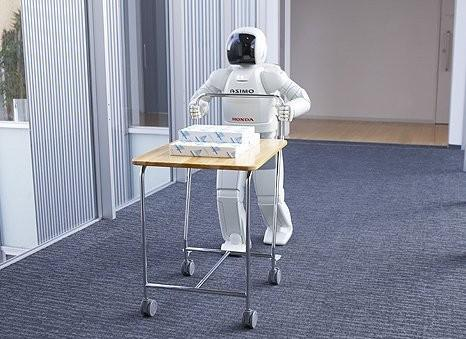
\includegraphics[scale=0.7]{images/StateOfArt/asimo.jpg}
			\caption{ASIMO pushing a cart}
			\label{asimo}
	\end{figure}
	\bigskip

Some of its aditional abilities include navigating space while avoiding oncoming people, carrying or pushing objects (Figure \ref{asimo}), using the stairs, playing sports such as soccer and heading towards its charging station whenever it detects its battery charge level is low.\\

\newpage
\subsection{RIBA}

The Robot for Interactive Body Assistance (RIBA) was developped in conjunction between RIKEN and Tokai Rubber Industries in the year 2004 to provide assistance in human handling, such as setting a person into thei wheelchair or transporting them to their bed.\\

The first RIBA, from 2009, could lift around 60kg, while the new RIBA II from 2011 is able to carry up to 80kg, which would cover most of Japan's population, the average adult weighing around 60kg.\\

Its 140cm height ensures it is able to lift people to the highest beds, while its 180kg provides a solid counterweight to avoid toppling over when carrying a person.\\

	\begin{figure}[H]
			\centering
			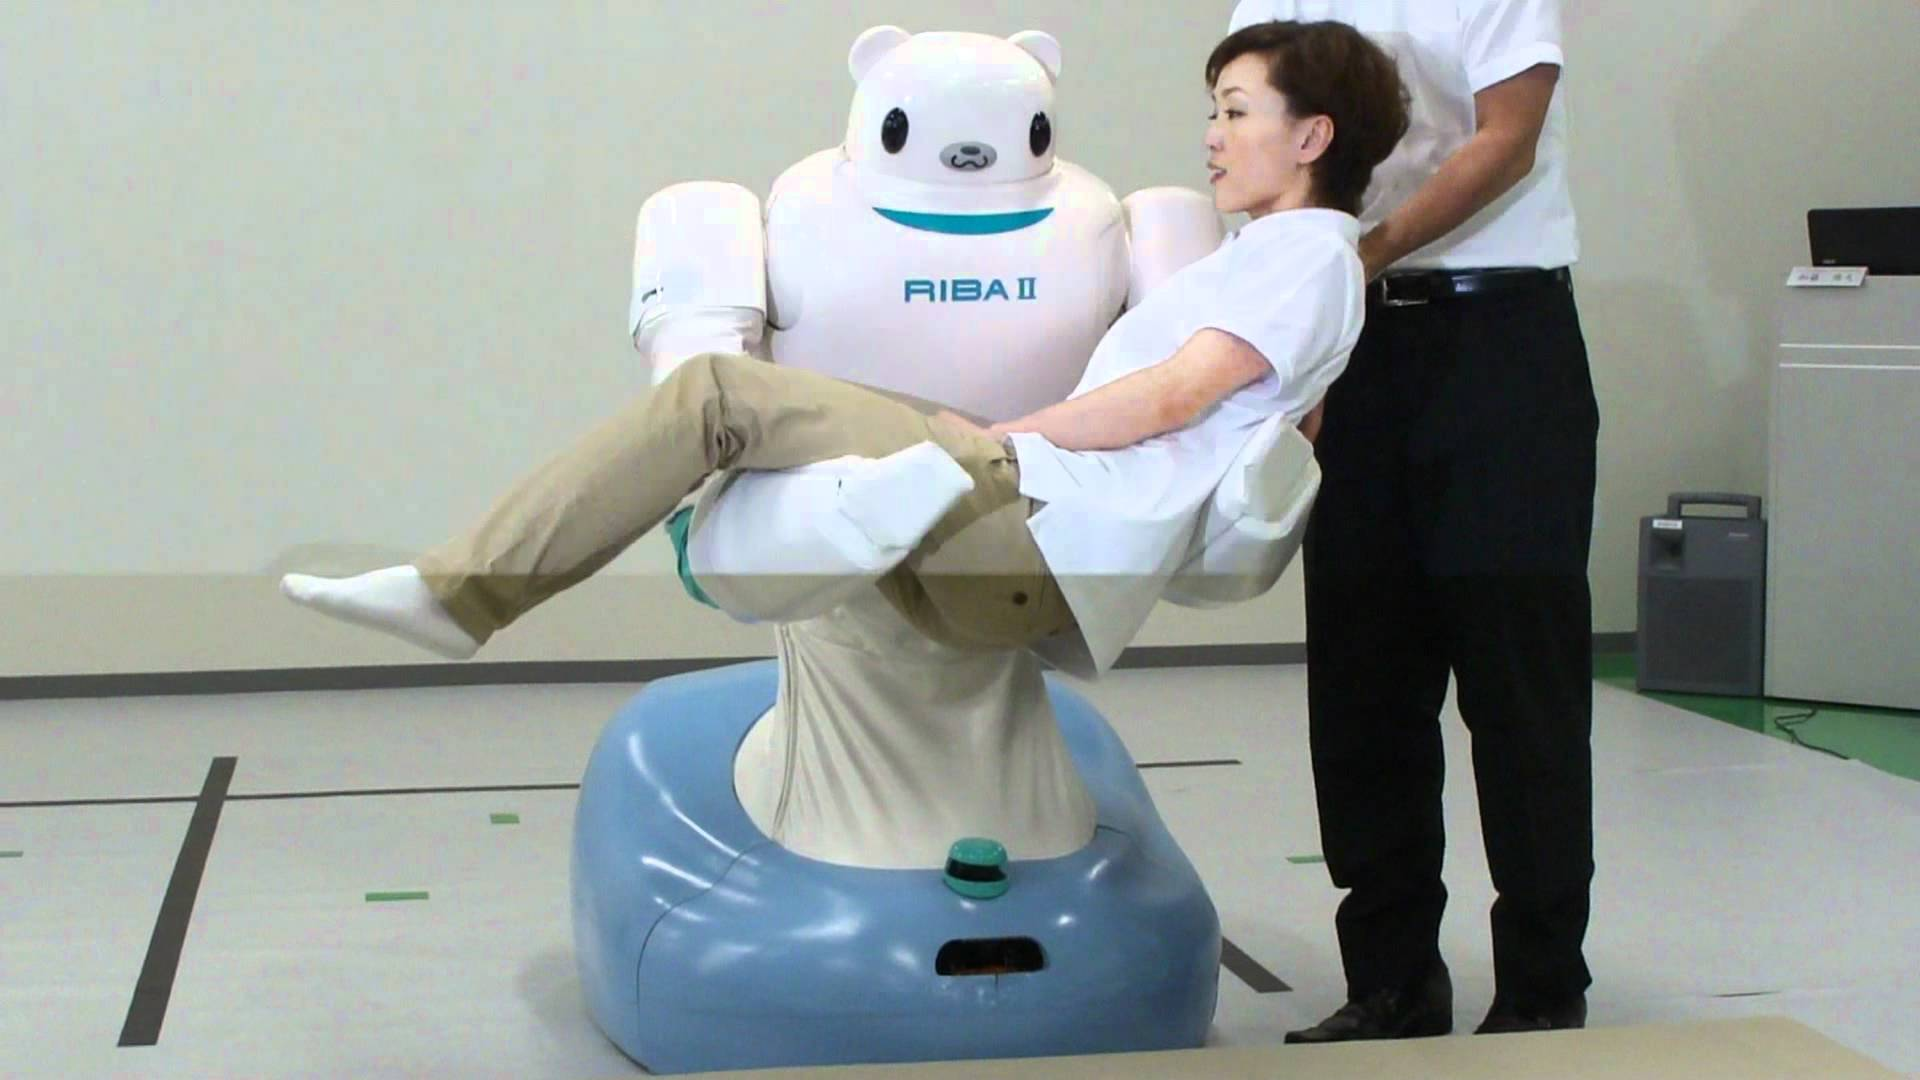
\includegraphics[scale=0.2]{images/StateOfArt/riba.jpg}
			\caption{RIBA II carrying a patient}
			\label{riba}
	\end{figure}
	\bigskip